\documentclass{standalone}
\usepackage{tikz}
\usetikzlibrary{patterns, positioning}


\begin{document}
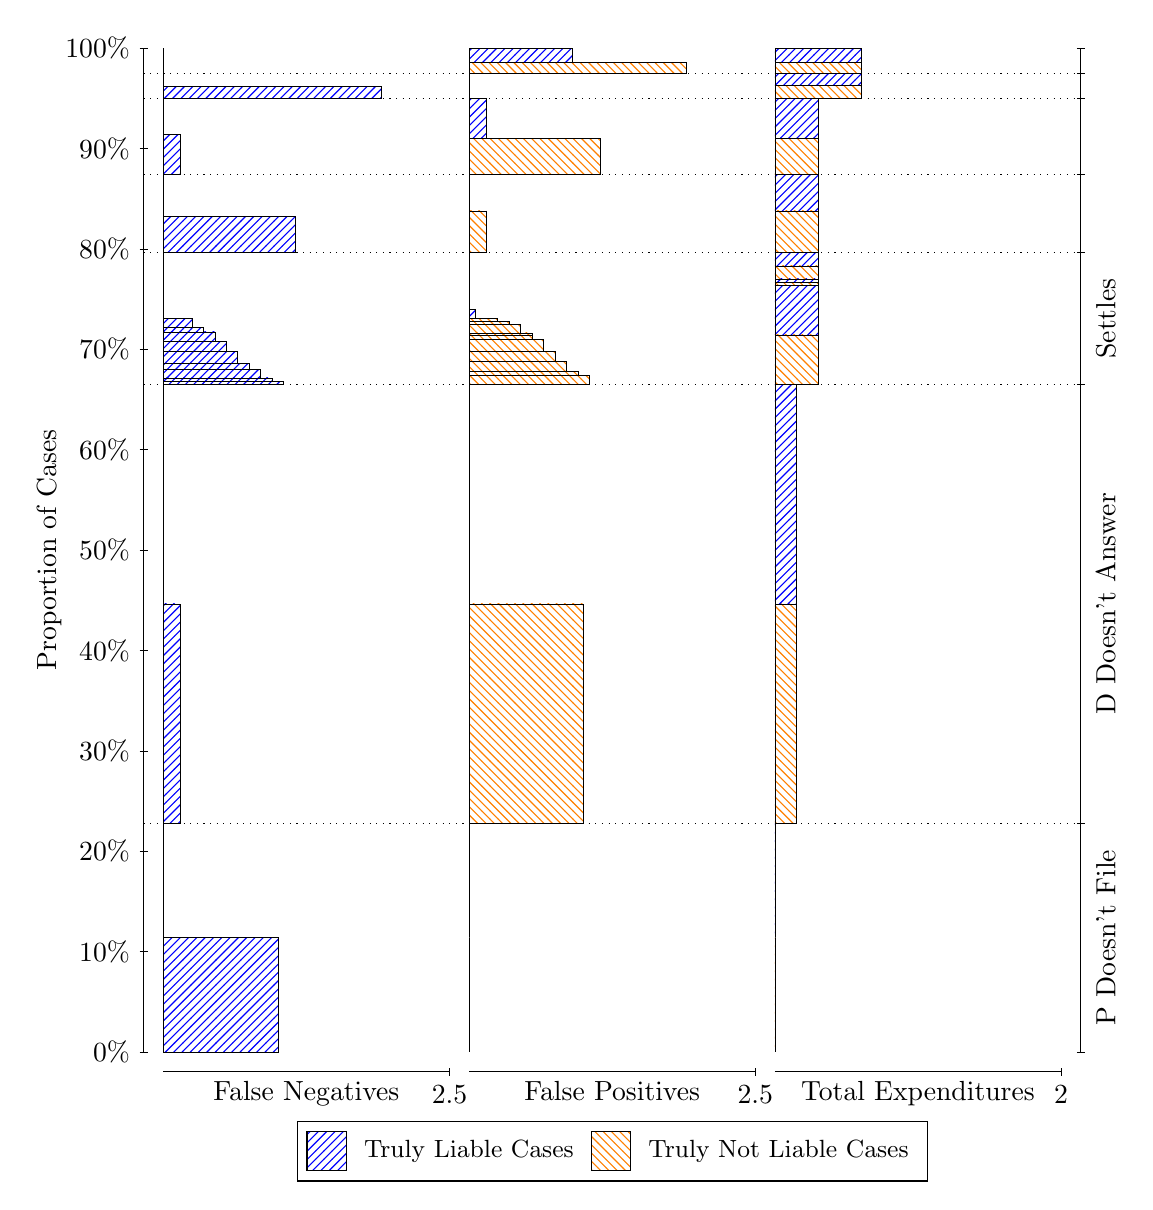
\begin{tikzpicture}
\draw[black, very thin] (1.5,1.75) -- (1.5,14.5);
\node[rotate=90, text=black, anchor=center] at (0.3, 8.125) {Proportion of Cases};
\draw[black, very thin] (1.45,1.75) -- (1.55,1.75);
\node[text=black, anchor=east] at (1.45, 1.75) {0\%};
\draw[black, very thin] (1.45,3.025) -- (1.55,3.025);
\node[text=black, anchor=east] at (1.45, 3.025) {10\%};
\draw[black, very thin] (1.45,4.3) -- (1.55,4.3);
\node[text=black, anchor=east] at (1.45, 4.3) {20\%};
\draw[black, very thin] (1.45,5.575) -- (1.55,5.575);
\node[text=black, anchor=east] at (1.45, 5.575) {30\%};
\draw[black, very thin] (1.45,6.85) -- (1.55,6.85);
\node[text=black, anchor=east] at (1.45, 6.85) {40\%};
\draw[black, very thin] (1.45,8.125) -- (1.55,8.125);
\node[text=black, anchor=east] at (1.45, 8.125) {50\%};
\draw[black, very thin] (1.45,9.4) -- (1.55,9.4);
\node[text=black, anchor=east] at (1.45, 9.4) {60\%};
\draw[black, very thin] (1.45,10.675) -- (1.55,10.675);
\node[text=black, anchor=east] at (1.45, 10.675) {70\%};
\draw[black, very thin] (1.45,11.95) -- (1.55,11.95);
\node[text=black, anchor=east] at (1.45, 11.95) {80\%};
\draw[black, very thin] (1.45,13.225) -- (1.55,13.225);
\node[text=black, anchor=east] at (1.45, 13.225) {90\%};
\draw[black, very thin] (1.45,14.5) -- (1.55,14.5);
\node[text=black, anchor=east] at (1.45, 14.5) {100\%};

\draw[black, very thin] (13.4,1.75) -- (13.4,14.5);
\draw[black, very thin] (13.35,1.75) -- (13.45,1.75);
\node[anchor=west] at (13.35, 1.75) {};
\draw[black, very thin] (13.35,4.6519) -- (13.45,4.6519);
\node[anchor=west] at (13.35, 4.6519) {};
\draw[black, very thin] (13.35,10.229) -- (13.45,10.229);
\node[anchor=west] at (13.35, 10.229) {};
\draw[black, very thin] (13.35,11.904) -- (13.45,11.904);
\node[anchor=west] at (13.35, 11.904) {};
\draw[black, very thin] (13.35,12.891) -- (13.45,12.891);
\node[anchor=west] at (13.35, 12.891) {};
\draw[black, very thin] (13.35,13.863) -- (13.45,13.863);
\node[anchor=west] at (13.35, 13.863) {};
\draw[black, very thin] (13.35,14.18) -- (13.45,14.18);
\node[anchor=west] at (13.35, 14.18) {};
\draw[black, very thin] (13.35,14.5) -- (13.45,14.5);
\node[anchor=west] at (13.35, 14.5) {};

\draw[black, very thin, pattern color=blue, pattern=north east lines] (1.75,1.75) rectangle (3.2033,3.2009);
\draw[black, very thin, pattern color=orange, pattern=north west lines] (1.75,3.2009) rectangle (1.75,4.6519);
\draw[black, very thin, pattern color=blue, pattern=north east lines] (1.75,4.6519) rectangle (1.968,7.4403);
\draw[black, very thin, pattern color=orange, pattern=north west lines] (1.75,7.4403) rectangle (1.75,10.229);
\draw[black, very thin, pattern color=blue, pattern=north east lines] (1.75,10.229) rectangle (3.276,10.271);
\draw[black, very thin, pattern color=blue, pattern=north east lines] (1.75,10.271) rectangle (3.1307,10.31);
\draw[black, very thin, pattern color=blue, pattern=north east lines] (1.75,10.31) rectangle (2.9853,10.415);
\draw[black, very thin, pattern color=blue, pattern=north east lines] (1.75,10.415) rectangle (2.84,10.495);
\draw[black, very thin, pattern color=blue, pattern=north east lines] (1.75,10.495) rectangle (2.6947,10.651);
\draw[black, very thin, pattern color=blue, pattern=north east lines] (1.75,10.651) rectangle (2.5493,10.77);
\draw[black, very thin, pattern color=blue, pattern=north east lines] (1.75,10.77) rectangle (2.404,10.896);
\draw[black, very thin, pattern color=blue, pattern=north east lines] (1.75,10.896) rectangle (2.2587,10.948);
\draw[black, very thin, pattern color=blue, pattern=north east lines] (1.75,10.948) rectangle (2.1133,11.065);
\draw[black, very thin, pattern color=orange, pattern=north west lines] (1.75,11.065) rectangle (1.75,11.904);
\draw[black, very thin, pattern color=blue, pattern=north east lines] (1.75,11.904) rectangle (3.4213,12.364);
\draw[black, very thin, pattern color=orange, pattern=north west lines] (1.75,12.364) rectangle (1.75,12.891);
\draw[black, very thin, pattern color=blue, pattern=north east lines] (1.75,12.891) rectangle (1.968,13.402);
\draw[black, very thin, pattern color=orange, pattern=north west lines] (1.75,13.402) rectangle (1.75,13.863);
\draw[black, very thin, pattern color=blue, pattern=north east lines] (1.75,13.863) rectangle (4.5113,14.014);
\draw[black, very thin, pattern color=orange, pattern=north west lines] (1.75,14.014) rectangle (1.75,14.18);
\draw[black, very thin, pattern color=orange, pattern=north west lines] (1.75,14.18) rectangle (1.75,14.322);
\draw[black, very thin, pattern color=blue, pattern=north east lines] (1.75,14.322) rectangle (1.75,14.5);
\draw[black, very thin, pattern color=orange, pattern=north west lines] (5.6333,1.75) rectangle (5.6333,3.2009);
\draw[black, very thin, pattern color=blue, pattern=north east lines] (5.6333,3.2009) rectangle (5.6333,4.6519);
\draw[black, very thin, pattern color=orange, pattern=north west lines] (5.6333,4.6519) rectangle (7.0867,7.4403);
\draw[black, very thin, pattern color=blue, pattern=north east lines] (5.6333,7.4403) rectangle (5.6333,10.229);
\draw[black, very thin, pattern color=orange, pattern=north west lines] (5.6333,10.229) rectangle (7.1593,10.341);
\draw[black, very thin, pattern color=orange, pattern=north west lines] (5.6333,10.341) rectangle (7.014,10.392);
\draw[black, very thin, pattern color=orange, pattern=north west lines] (5.6333,10.392) rectangle (6.8687,10.52);
\draw[black, very thin, pattern color=orange, pattern=north west lines] (5.6333,10.52) rectangle (6.7233,10.643);
\draw[black, very thin, pattern color=orange, pattern=north west lines] (5.6333,10.643) rectangle (6.578,10.803);
\draw[black, very thin, pattern color=orange, pattern=north west lines] (5.6333,10.803) rectangle (6.4327,10.858);
\draw[black, very thin, pattern color=orange, pattern=north west lines] (5.6333,10.858) rectangle (6.4327,10.883);
\draw[black, very thin, pattern color=orange, pattern=north west lines] (5.6333,10.883) rectangle (6.2873,10.987);
\draw[black, very thin, pattern color=orange, pattern=north west lines] (5.6333,10.987) rectangle (6.142,11.025);
\draw[black, very thin, pattern color=orange, pattern=north west lines] (5.6333,11.025) rectangle (5.9967,11.068);
\draw[black, very thin, pattern color=blue, pattern=north east lines] (5.6333,11.068) rectangle (5.706,11.185);
\draw[black, very thin, pattern color=blue, pattern=north east lines] (5.6333,11.185) rectangle (5.6333,11.904);
\draw[black, very thin, pattern color=orange, pattern=north west lines] (5.6333,11.904) rectangle (5.8513,12.431);
\draw[black, very thin, pattern color=blue, pattern=north east lines] (5.6333,12.431) rectangle (5.6333,12.891);
\draw[black, very thin, pattern color=orange, pattern=north west lines] (5.6333,12.891) rectangle (7.3047,13.352);
\draw[black, very thin, pattern color=blue, pattern=north east lines] (5.6333,13.352) rectangle (5.8513,13.863);
\draw[black, very thin, pattern color=orange, pattern=north west lines] (5.6333,13.863) rectangle (5.6333,14.029);
\draw[black, very thin, pattern color=blue, pattern=north east lines] (5.6333,14.029) rectangle (5.6333,14.18);
\draw[black, very thin, pattern color=orange, pattern=north west lines] (5.6333,14.18) rectangle (8.3947,14.322);
\draw[black, very thin, pattern color=blue, pattern=north east lines] (5.6333,14.322) rectangle (6.9413,14.5);
\draw[black, very thin, pattern color=orange, pattern=north west lines] (9.5167,1.75) rectangle (9.5167,3.2009);
\draw[black, very thin, pattern color=blue, pattern=north east lines] (9.5167,3.2009) rectangle (9.5167,4.6519);
\draw[black, very thin, pattern color=orange, pattern=north west lines] (9.5167,4.6519) rectangle (9.7892,7.4403);
\draw[black, very thin, pattern color=blue, pattern=north east lines] (9.5167,7.4403) rectangle (9.7892,10.229);
\draw[black, very thin, pattern color=orange, pattern=north west lines] (9.5167,10.229) rectangle (10.062,10.858);
\draw[black, very thin, pattern color=blue, pattern=north east lines] (9.5167,10.858) rectangle (10.062,11.483);
\draw[black, very thin, pattern color=orange, pattern=north west lines] (9.5167,11.483) rectangle (10.062,11.526);
\draw[black, very thin, pattern color=blue, pattern=north east lines] (9.5167,11.526) rectangle (10.062,11.568);
\draw[black, very thin, pattern color=orange, pattern=north west lines] (9.5167,11.568) rectangle (10.062,11.734);
\draw[black, very thin, pattern color=blue, pattern=north east lines] (9.5167,11.734) rectangle (10.062,11.904);
\draw[black, very thin, pattern color=orange, pattern=north west lines] (9.5167,11.904) rectangle (10.062,12.431);
\draw[black, very thin, pattern color=blue, pattern=north east lines] (9.5167,12.431) rectangle (10.062,12.891);
\draw[black, very thin, pattern color=orange, pattern=north west lines] (9.5167,12.891) rectangle (10.062,13.352);
\draw[black, very thin, pattern color=blue, pattern=north east lines] (9.5167,13.352) rectangle (10.062,13.863);
\draw[black, very thin, pattern color=orange, pattern=north west lines] (9.5167,13.863) rectangle (10.607,14.029);
\draw[black, very thin, pattern color=blue, pattern=north east lines] (9.5167,14.029) rectangle (10.607,14.18);
\draw[black, very thin, pattern color=orange, pattern=north west lines] (9.5167,14.18) rectangle (10.607,14.322);
\draw[black, very thin, pattern color=blue, pattern=north east lines] (9.5167,14.322) rectangle (10.607,14.5);
\draw[black, dotted] (1.5,4.6519) -- (13.4,4.6519);
\draw[black, dotted] (1.5,10.229) -- (13.4,10.229);
\draw[black, dotted] (1.5,11.904) -- (13.4,11.904);
\draw[black, dotted] (1.5,12.891) -- (13.4,12.891);
\draw[black, dotted] (1.5,13.863) -- (13.4,13.863);
\draw[black, dotted] (1.5,14.18) -- (13.4,14.18);
\draw[black, very thin] (1.75,1.5) -- (5.3833,1.5);
\node[text=black, anchor=north] at (3.5667, 1.5) {False Negatives};
\draw[black, very thin] (5.3833,1.45) -- (5.3833,1.55);
\node[text=black, anchor=north] at (5.3833, 1.45) {2.5};

\draw[black, very thin] (5.6333,1.5) -- (9.2667,1.5);
\node[text=black, anchor=north] at (7.45, 1.5) {False Positives};
\draw[black, very thin] (9.2667,1.45) -- (9.2667,1.55);
\node[text=black, anchor=north] at (9.2667, 1.45) {2.5};

\draw[black, very thin] (9.5167,1.5) -- (13.15,1.5);
\node[text=black, anchor=north] at (11.333, 1.5) {Total Expenditures};
\draw[black, very thin] (13.15,1.45) -- (13.15,1.55);
\node[text=black, anchor=north] at (13.15, 1.45) {2};

\node[text=black, centered, rotate=90] at (13.72, 3.2009) {P Doesn't File};
\node[text=black, centered, rotate=90] at (13.72, 7.4403) {D Doesn't Answer};
\node[text=black, centered, rotate=90] at (13.72, 11.066) {Settles};





\draw (7.449999999999999,1.5) node[draw=none] (baseCoordinate) {};
\begin{scope}[align=center]
        \matrix[scale=0.5, draw=black, below=0.5cm of baseCoordinate, nodes={draw}, column sep=0.1cm]{
            \node[rectangle, draw, minimum width=0.5cm, minimum height=0.5cm, pattern color=blue, pattern=north east lines] {}; &
            \node[draw=none, font=\small, text=black] (B) {Truly Liable Cases}; &
            \node[rectangle, draw, minimum width=0.5cm, minimum height=0.5cm, pattern color=orange, pattern=north west lines] {}; &
            \node[draw=none, font=\small, text=black] (B) {Truly Not Liable Cases}; \\
            };
\end{scope}

\end{tikzpicture}
\end{document}